\section{Introduction}

\subsection{Task Definition}
As part of the course "Parallel Systems" we were given the task of implementing an algorithm that generates a voronoi diagram and then parallelizing this algorithm with two different frameworks. In this paper we will first explain briefly what voronoi diagrams are and what practical uses they have. Then we will go into the implementation and explanation of, first, our algorithm without any parallelization, second, the parallelization using OpenMP and third, the parallelization using OpenMPI. Finally, we will present, on one hand, the process by which we define and control the benchmarks and on the other hand, the results and comparisons of said benchmarks.

\subsection{Voronoi-Diagrams}
voronoi Diagrams allow the tesselation of planes into different areas using a very intuitive and simple principle: Given a finite set of points on a plane, called centroids, a region formed by all the points that are closer to one centroid than to all other centroids on the plane, is assigned to said centroid. In other words, what this diagram does is to divide the plane into as many regions as we have centroids, in such a way that we assign to each centroid the region formed by everything that is closer to it than to any other. If you then assign a unique color to each centroid, and color each point respectively to it’s closest centroid, a visual representation (see \ref{fig:voronoi-diagram}) can be created in order to display the created cells.

\begin{center}
    \begin{figure}[H]
        \centering
            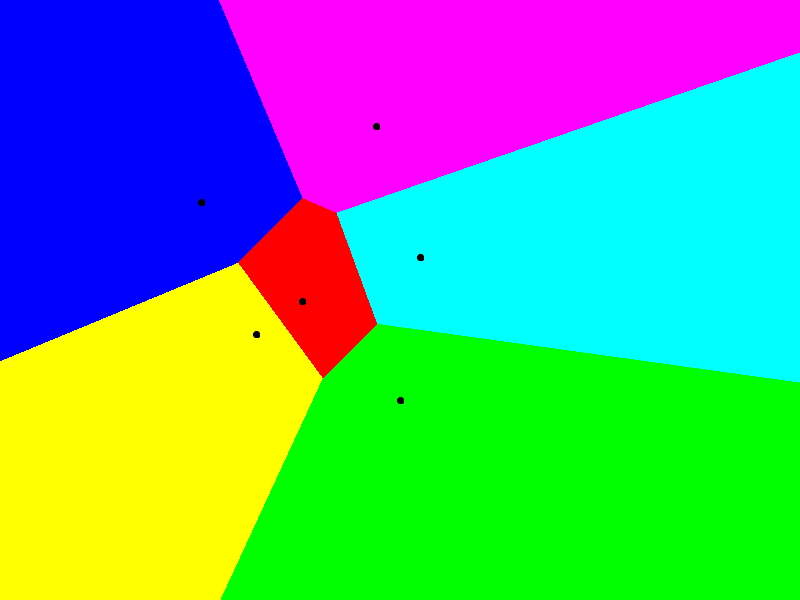
\includegraphics[width=8cm]{resources/images/introduction/voronoi.png}
            \caption{Voronoi-Diagramm}
            \label{fig:voronoi-diagram}
    \end{figure}
\end{center}

\subsubsection{Delauney-Triangulation}

There are different ways of calculating and generating voronoi diagrams. One option is using brute force and iterating every point on the plane in order to find the closest centroid, which works and is a straight forward, easy to understand solution but does not scale well, as bigger planes will require much more computational power and time. Another, more performant solution is the so called Delauney triangulation. 
A triangulation, as the name suggests, is the division of a plane into smaller triangles. What distinguishes the Delauney triangulation is that all the triangles in this particular triangulation must fulfill the Delauney condition. For a triangle to meet this condition, a circle is drawn where the three corners of the triangle lie on its circumference (see \ref{fig:brokenDelauneyCondition}). If there is a corner of another triangle within this circle, then Delauney's condition is not fulfilled and the triangle must be discarded. But as long as no other corner is found inside the circumference, besides the three corners of the initial triangle (see \ref{fig:metDelauneyCondition}), the condition is fulfilled and the triangle may belong to the tesselation of the surface.

\begin{center}
    \begin{figure}[H]
        \centering
        \begin{subfigure}[b]{0.45\textwidth}
            \centering
            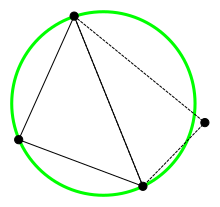
\includegraphics[width=\textwidth]{resources/images/introduction/Point_outside_circle.png}
            \caption{Broken delauney condition}
            \label{fig:brokenDelauneyCondition}
        \end{subfigure}
        \hfill
        \begin{subfigure}[b]{0.45\textwidth}
            \centering
            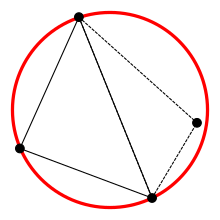
\includegraphics[width=\textwidth]{resources/images/introduction/Point_inside_circle.png}
            \caption{Met delauney condition}
            \label{fig:metDelauneyCondition}
        \end{subfigure}
        \caption{Visualization of the delauney condition}
        \label{fig:delauneyCondition}
    \end{figure}
\end{center}

Once the Delauney triangulation is calculated, the surface has been tessellated by triangles, as can be seen in the image \ref{fig:delauneyTriangulation}, and the centers of the circles belonging to each triangle, marked in red in the image, are known. With this information, a voronoi diagram can be readily produced, since this triangulation represents the dual graph of the voronoi diagram. That is, the centers of the circles represent the vertices of the voronoi diagram and they are connected to each other, if their corresponding triangles share an edge (see \ref{fig:delauneyVoronoi}).

\begin{center}
    \begin{figure}[H]
        \centering
        \begin{subfigure}[b]{0.45\textwidth}
            \centering
            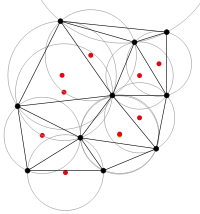
\includegraphics[width=\textwidth]{resources/images/introduction/Delaunay_circumcircles_centers.svg.png}
            \caption{Delauney triangulation}
            \label{fig:delauneyTriangulation}
        \end{subfigure}
        \hfill
        \begin{subfigure}[b]{0.45\textwidth}
            \centering
            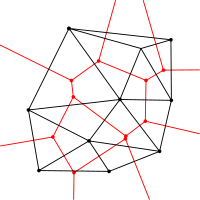
\includegraphics[width=\textwidth]{resources/images/introduction/Delaunay_Voronoi.svg.png}
            \caption{Resulting voronoi diagram}
            \label{fig:delauneyVoronoi}
        \end{subfigure}
        \caption{Relationship between delauney triangulations and voronoi diagrams}
        \label{fig:delauneyVoronoi}
    \end{figure}
\end{center}

\subsubsection{Use Cases}

The practical uses of voronoi diagrams cover a wide spectrum of areas, ranging from city planning to computer science, medicine, engineering and many more.\\

A concrete example is the use of voronoi Diagrams to solve the nearest-neighbour-problem. For example, if a voronoi diagram is created, using certain points of interest as centroids, for example hospitals, and a person wants to reach the closest one to their current position, it is only necessary to determine in which region of the voronoi diagram the person is currently located and thus the centroid of this region is the closest hospital. The images below, show a sample situation, where the hospitals and the position of the person are mapped (see \ref{fig:mappedHospitals}), and using a voronoi tesselation, it can be determined that the closest hospital is the one located in the maroon area (see \ref{fig:hospitalVoron}). 

\begin{center}
    \begin{figure}[H]
        \centering
        \begin{subfigure}[b]{0.45\textwidth}
            \centering
            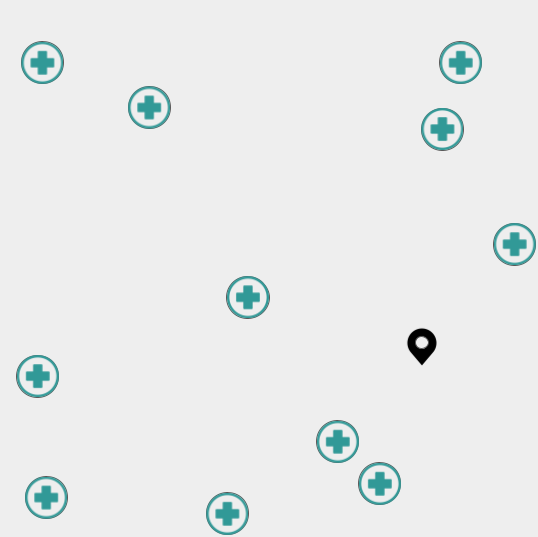
\includegraphics[width=\textwidth]{resources/images/introduction/HospitalNoVoronoi.png}
            \caption{Mapped hospitals}
            \label{fig:mappedHospitals}
        \end{subfigure}
        \hfill
        \begin{subfigure}[b]{0.45\textwidth}
            \centering
            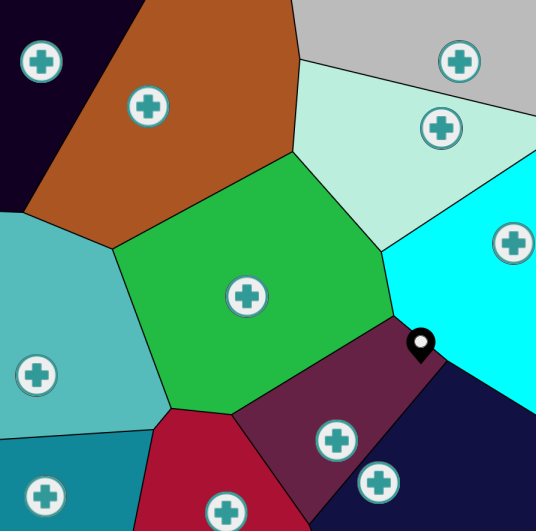
\includegraphics[width=\textwidth]{resources/images/introduction/HospitalVoronoi.png}
            \caption{Hospital voronoi diagram}
            \label{fig:hospitalVoronoi}
        \end{subfigure}
        \caption{Voronoi use case - Closest hospital}
        \label{fig:voronoiUseCase}
    \end{figure}
\end{center}